\documentclass{article} % Starts an article
\usepackage{tikz}
\usetikzlibrary{shapes.geometric, arrows, calc}
\usepackage[numbib]{tocbibind}
\tikzstyle{cool} = [rectangle, rounded corners, minimum width=3cm, minimum
height=1cm, text centered, draw=black, fill=gray!30, text width=3cm]
\tikzstyle{arrow} = [thick, ->, >=stealth]
\tikzstyle{line} = [thick, -, >=stealth]


\begin{document}



\tikzstyle{cool} = [rectangle, rounded corners, minimum width=3cm, minimum
height=1cm, text centered, draw=black, fill=gray!30, text width=3cm]
\tikzstyle{arrow} = [thick, ->, >=stealth]
\tikzstyle{line} = [thick, -, >=stealth]

\begin{figure}
    \centering
    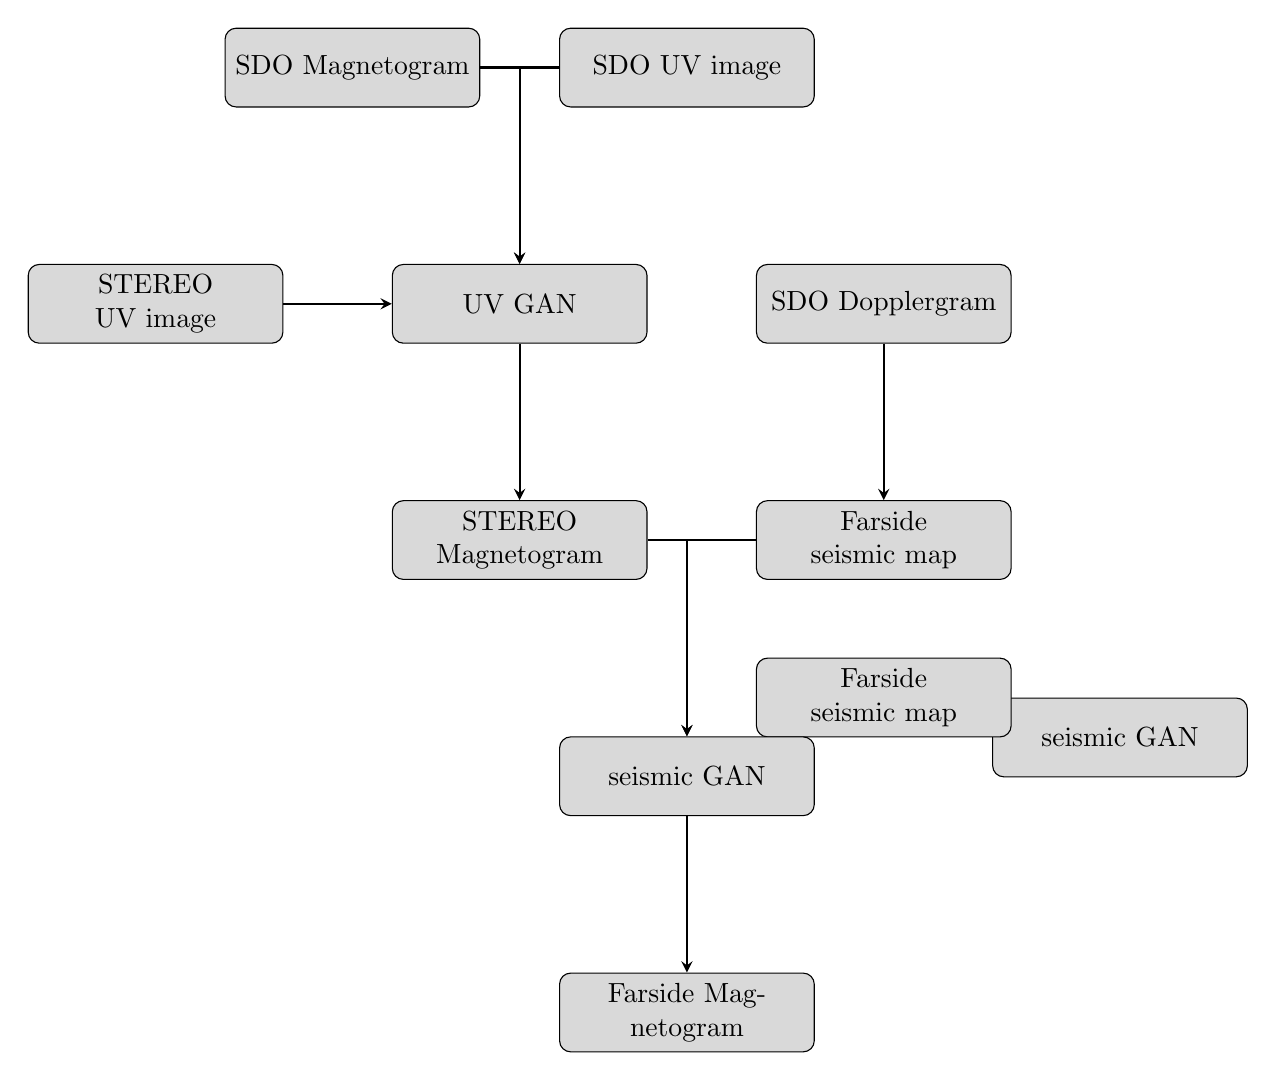
\begin{tikzpicture}[node distance=3cm]
        % \draw[help lines] (0,-5) grid (10,10);
        
        \node (SGAN) [cool, right=6cm] {seismic GAN};
        \node (FS) [cool, left of=SGAN, above=0cm] {Farside\\ seismic map};




        \node (UVGAN) [cool, above=5cm] {UV GAN};
        \node (STEU) [cool, left of=UVGAN, left=0cm] {STEREO UV image};
        \node (SDOD) [cool, right of=UVGAN, right=0cm] {SDO Dopplergram};

        \node (SDOM) [cool, above of=UVGAN, left=0.5cm] {SDO Magnetogram};
        \node (SDOU) [cool, above of=UVGAN, right=0.5cm] {SDO UV image};

        \node (STEM) [cool, below of=UVGAN] {STEREO Magnetogram};
        \node (FS) [cool, right of=STEM, right=0cm] {Farside\\ seismic map};

        \node (SGAN) [cool, below of=STEM, right=0.5cm] {seismic GAN};
        \node (FM) [cool, below of=SGAN] {Farside Magnetogram};
        
        \draw [arrow] (SDOU) -| node[anchor=south] {} (UVGAN);
        \draw [arrow] (SDOM) -| node[anchor=south] {} (UVGAN);

        \draw [arrow] (STEU) -- node[anchor=east] {} (UVGAN);

        \draw [arrow] (UVGAN) -- node[anchor=south] {} (STEM);
        \draw [arrow] (SDOD) -- node[anchor=south] {} (FS);

        \draw [arrow] (STEM) -| node[anchor=south] {} (SGAN);
        \draw [arrow] (FS) -| node[anchor=south] {} (SGAN);

        \draw [arrow] (SGAN) -_ node[anchor=south] {} (FM);

        % \coordinate (SU) at ([yshift=-1cm]SDOU.south); % we collect the edges in front of Q
        % \coordinate (SM) at ([yshift=-1cm]SDOM.south); % we collect the edges in front of Q
        % \coordinate (UU) at ([]UVGAN.north); % we collect the edges in front of Q
        % \draw [line] (SDOU) -|  (SU);
        % \draw [line] (SDOM) -|  (SM);
        % \draw [line] (SU) -|  (UU);
        % \draw [line] (SM) -|  (UU);


        % \draw [arrow] (D) -- node[anchor=south, text width=2cm] {Helioseismic Holography} (P);
        % \draw [arrow] (MM) -- node[anchor=south] {Train} (M);
        % \draw [line] (P) -|  (FF);
        % \draw [line] (N) -|  (FF);
        % \draw [line] (S) -|  (MM);
        % \draw [line] (E) -|  (MM);
        % \draw [arrow] (FF) -- node[anchor=south] {cGAN} (F);
        % \draw [arrow] (Q) -- node[anchor=south, text width=2cm] {} (M);


        % \node (E) [cool] {SDO UV image};
        % \node (M) [cool, right of=E, below=0.5cm] {UV GAN};
        % \node (N) [cool, right of=M] {STEREO Magnetogram};
        % \node (D) [cool, right of=E, above=0.5cm] {SDO Dopplergram};
        % \node (P) [cool, right of=D] {Farside \quad \quad \quad \qquad  seismic map};
        % \node (F) [cool, right of=N, above=0.5cm] {Farside\\ Magnetogram};
        % % \node (S) [cool, below=1.5cm] {SDO Magnetogram};
        % \node (Q) [cool, right of=S, below=0.5cm] {STEREO UV image};





    \end{tikzpicture}
    \caption{Test}
\end{figure}


\end{document}
